\documentclass[tikz, border=2mm, dvipsnames, table]{standalone}

\usepackage[]{xcolor}
\usepackage{tikz-timing}
\usetikztiminglibrary{advnodes}
\usepackage{tcolorbox}
\usetikzlibrary{positioning}
\usepackage{amsmath}


\colorlet{networkheadercolor_base}{ForestGreen}
\colorlet{networkheadercolor}{networkheadercolor_base!30}
\colorlet{payloadcolor_base}{RoyalBlue}
\colorlet{payloadcolor}{payloadcolor_base!30}
\colorlet{idcolor_base}{Orange}
\colorlet{idcolor}{idcolor_base!40}

\newcommand*\circled[1]{\tikz[baseline=(char.base)]{
            \node[shape=rectangle,draw,inner sep=0pt, minimum size=4mm] (char) {\scriptsize #1};}}

\begin{document}
\begin{tikzpicture}
\node (table) at (0,0) {
\begin{tikztimingtable}[timing/.style={x=1cm,y=0.5cm}, x=2cm, y=0.5cm]
Standard frame & LN(A0);
[fill=networkheadercolor]D{NH}N(B0)D{L}N(C0);
[fill=payloadcolor]3D{Payload}N(E0);
[]L\\\\
Error frame & LN(A1);
[fill=networkheadercolor]D{NH}N(B1)D{err. code}N(C1);
[]L\\\\
Hop frame & LN(A);
[fill=networkheadercolor]D{NH}N(B)D{L}N(C);
[fill=idcolor]D{AH}N(D)2D{ID}N(E);
[fill=payloadcolor]3D{Payload}N(G);
[]L\\
\extracode
\node[anchor=north] at ($(A0.low2)!0.5!(B0.low)$) {\scriptsize 1};
\node[anchor=north] at ($(B0.low2)!0.5!(C0.low)$) {\scriptsize 2};
\node[anchor=north] at ($(C0.low2)!0.5!(E0.low2)$) {\scriptsize L};

\draw[networkheadercolor_base,|-|] ($(A0.mid)+(0.01,-2)$) -- ($(C0.mid)+(-0.01,-2)$) node[midway,anchor=north] {\circled{H}};
\draw[payloadcolor_base,|-|] ($(C0.mid)+(0.01,-2)$) -- ($(E0.mid)+(-0.01,-2)$) node[midway,anchor=north] {\circled{P}};

\draw[networkheadercolor_base,|-|] ($(A1.mid)+(0.01,-2)$) -- ($(C1.mid)+(-0.01,-2)$) node[midway,anchor=north] {\circled{H}};
\node[anchor=north] at ($(A1.low2)!0.5!(B1.low)$) {\scriptsize 1};
\node[anchor=north] at ($(B1.low2)!0.5!(C1.low2)$) {\scriptsize 2};

\draw[networkheadercolor_base,|-|] ($(A.mid)+(0.01,-2)$) -- ($(C.mid)+(-0.01,-2)$) node[midway,anchor=north] {\circled{H}};
\draw[idcolor_base,|-|] ($(C.mid)+(0.01,-2)$) -- ($(E.mid)+(-0.01,-2)$) node[midway,anchor=north] {\circled{I}};
\draw[payloadcolor_base,|-|] ($(E.mid)+(0.01,-2)$) -- ($(G.mid)+(-0.01,-2)$) node[midway,anchor=north] {\circled{P}};

\end{tikztimingtable}};



\tcbset
    {
        left=1mm,
        right=1mm,
        height=4mm,
        valign=center,
        boxrule=0.4pt,
        colframe=black,
    }
    
\node[anchor=north] at (table.south) {\sffamily\tiny
\tcbox[colback=networkheadercolor]{NH : Network header}
\tcbox[colback=networkheadercolor]{L : Frame length}
\tcbox[colback=idcolor]{AH : Addressing header}
\tcbox[colback=idcolor]{ID : Addressing ID}
};

\end{tikzpicture}

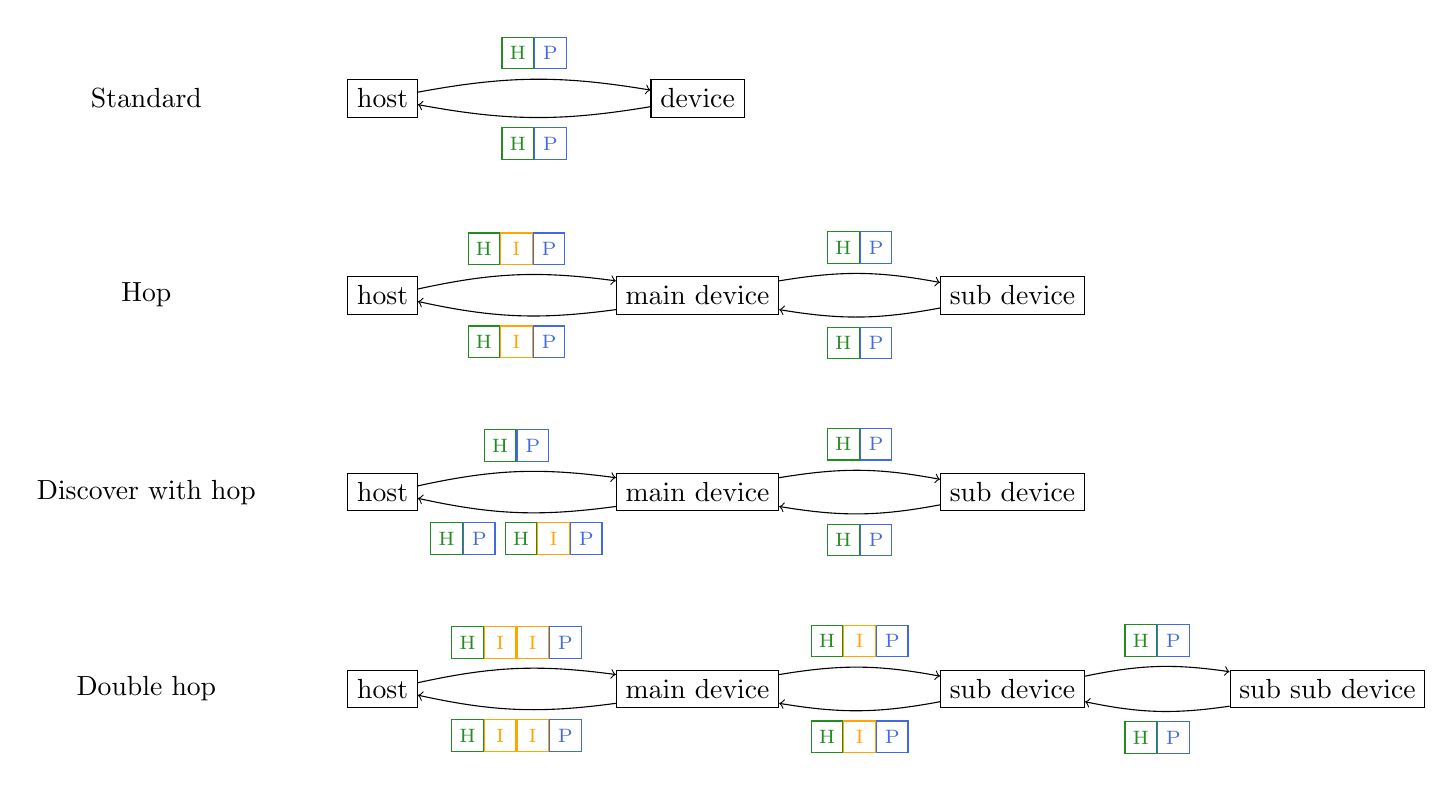
\begin{tikzpicture}
\tikzstyle{host}=[rectangle,draw]
\tikzstyle{device}=[rectangle,draw]
\tikzstyle{description}=[]
\tikzstyle{arrow}=[->,bend left=10]
\def\sdesc{-3}
\def\sd{4}
\def\vsep{-2.5}
\def\H{\textcolor{networkheadercolor_base}{\circled{H}}}
\def\I{\textcolor{idcolor_base}{\circled{I}}}
\def\C{\textcolor{cmdcolor_base}{\circled{C}}}
\def\P{\textcolor{payloadcolor_base}{\circled{P}}}



\node[description] (D1) at (\sdesc,0) {Standard};
\node[host] (H1) at (0,0) {host};
\node[device] (D1) at (\sd,0) {device};
\draw[->] (H1) to[arrow] node[midway,anchor=south] {\H\P} (D1);
\draw[->] (D1) to[arrow] node[midway,anchor=north] {\H\P} (H1);


\node[description] (D1) at (\sdesc,\vsep) {Hop};
\node[host] (H1) at (0,\vsep) {host};
\node[device] (D1) at (\sd,\vsep) {main device};
\node[device] (D2) at ({\sd*2},\vsep) {sub device};
\draw[->] (H1) to[arrow] node[midway,anchor=south] {\H\I\P} (D1);
\draw[->] (D1) to[arrow] node[midway,anchor=south] {\H\P} (D2);
\draw[->] (D2) to[arrow] node[midway,anchor=north] {\H\P} (D1);
\draw[->] (D1) to[arrow] node[midway,anchor=north] {\H\I\P} (H1);


\node[description] (D1) at (\sdesc,{\vsep*2}) {Discover with hop};
\node[host] (H1) at (0,{\vsep*2}) {host};
\node[device] (D1) at (\sd,{\vsep*2}) {main device};
\node[device] (D2) at ({\sd*2},{\vsep*2}) {sub device};
\draw[->] (H1) to[arrow] node[midway,anchor=south] {\H\P} (D1);
\draw[->] (D1) to[arrow] node[midway,anchor=south] {\H\P} (D2);
\draw[->] (D2) to[arrow] node[midway,anchor=north] {\H\P} (D1);
\draw[->] (D1) to[arrow] node[midway,anchor=north] {\H\P\ \H\I\P} (H1);

\node[description] (D1) at (\sdesc,{\vsep*3}) {Double hop};
\node[host] (H1) at (0,{\vsep*3}) {host};
\node[device] (D1) at (\sd,{\vsep*3}) {main device};
\node[device] (D2) at ({\sd*2},{\vsep*3}) {sub device};
\node[device] (D3) at ({\sd*3},{\vsep*3}) {sub sub device};
\draw[->] (H1) to[arrow] node[midway,anchor=south] {\H\I\I\P} (D1);
\draw[->] (D1) to[arrow] node[midway,anchor=south] {\H\I\P} (D2);
\draw[->] (D2) to[arrow] node[midway,anchor=south] {\H\P} (D3);
\draw[->] (D3) to[arrow] node[midway,anchor=north] {\H\P} (D2);
\draw[->] (D2) to[arrow] node[midway,anchor=north] {\H\I\P} (D1);
\draw[->] (D1) to[arrow] node[midway,anchor=north] {\H\I\I\P} (H1);
\end{tikzpicture}

\end{document}


